\FloatBarrier
\subsection{Euclidean distances analysis for Zernike modes PSFs}

	\subsubsection{Preprocessing}
		
		\begin{itemize}
			\item The PSF electric fields matrices are flattened to compute the euclidean distances between 1d vectors.
			\item 70000 datapoint pairs for each zernike datasets are randomly defined. The euclidean distances will be calculated for these selected pairs.
			\item In this case, LP coefficients are also analysed.
		\end{itemize}
			
	\subsubsection{Results}
		\begin{figure*}[ht!]
			\centering
			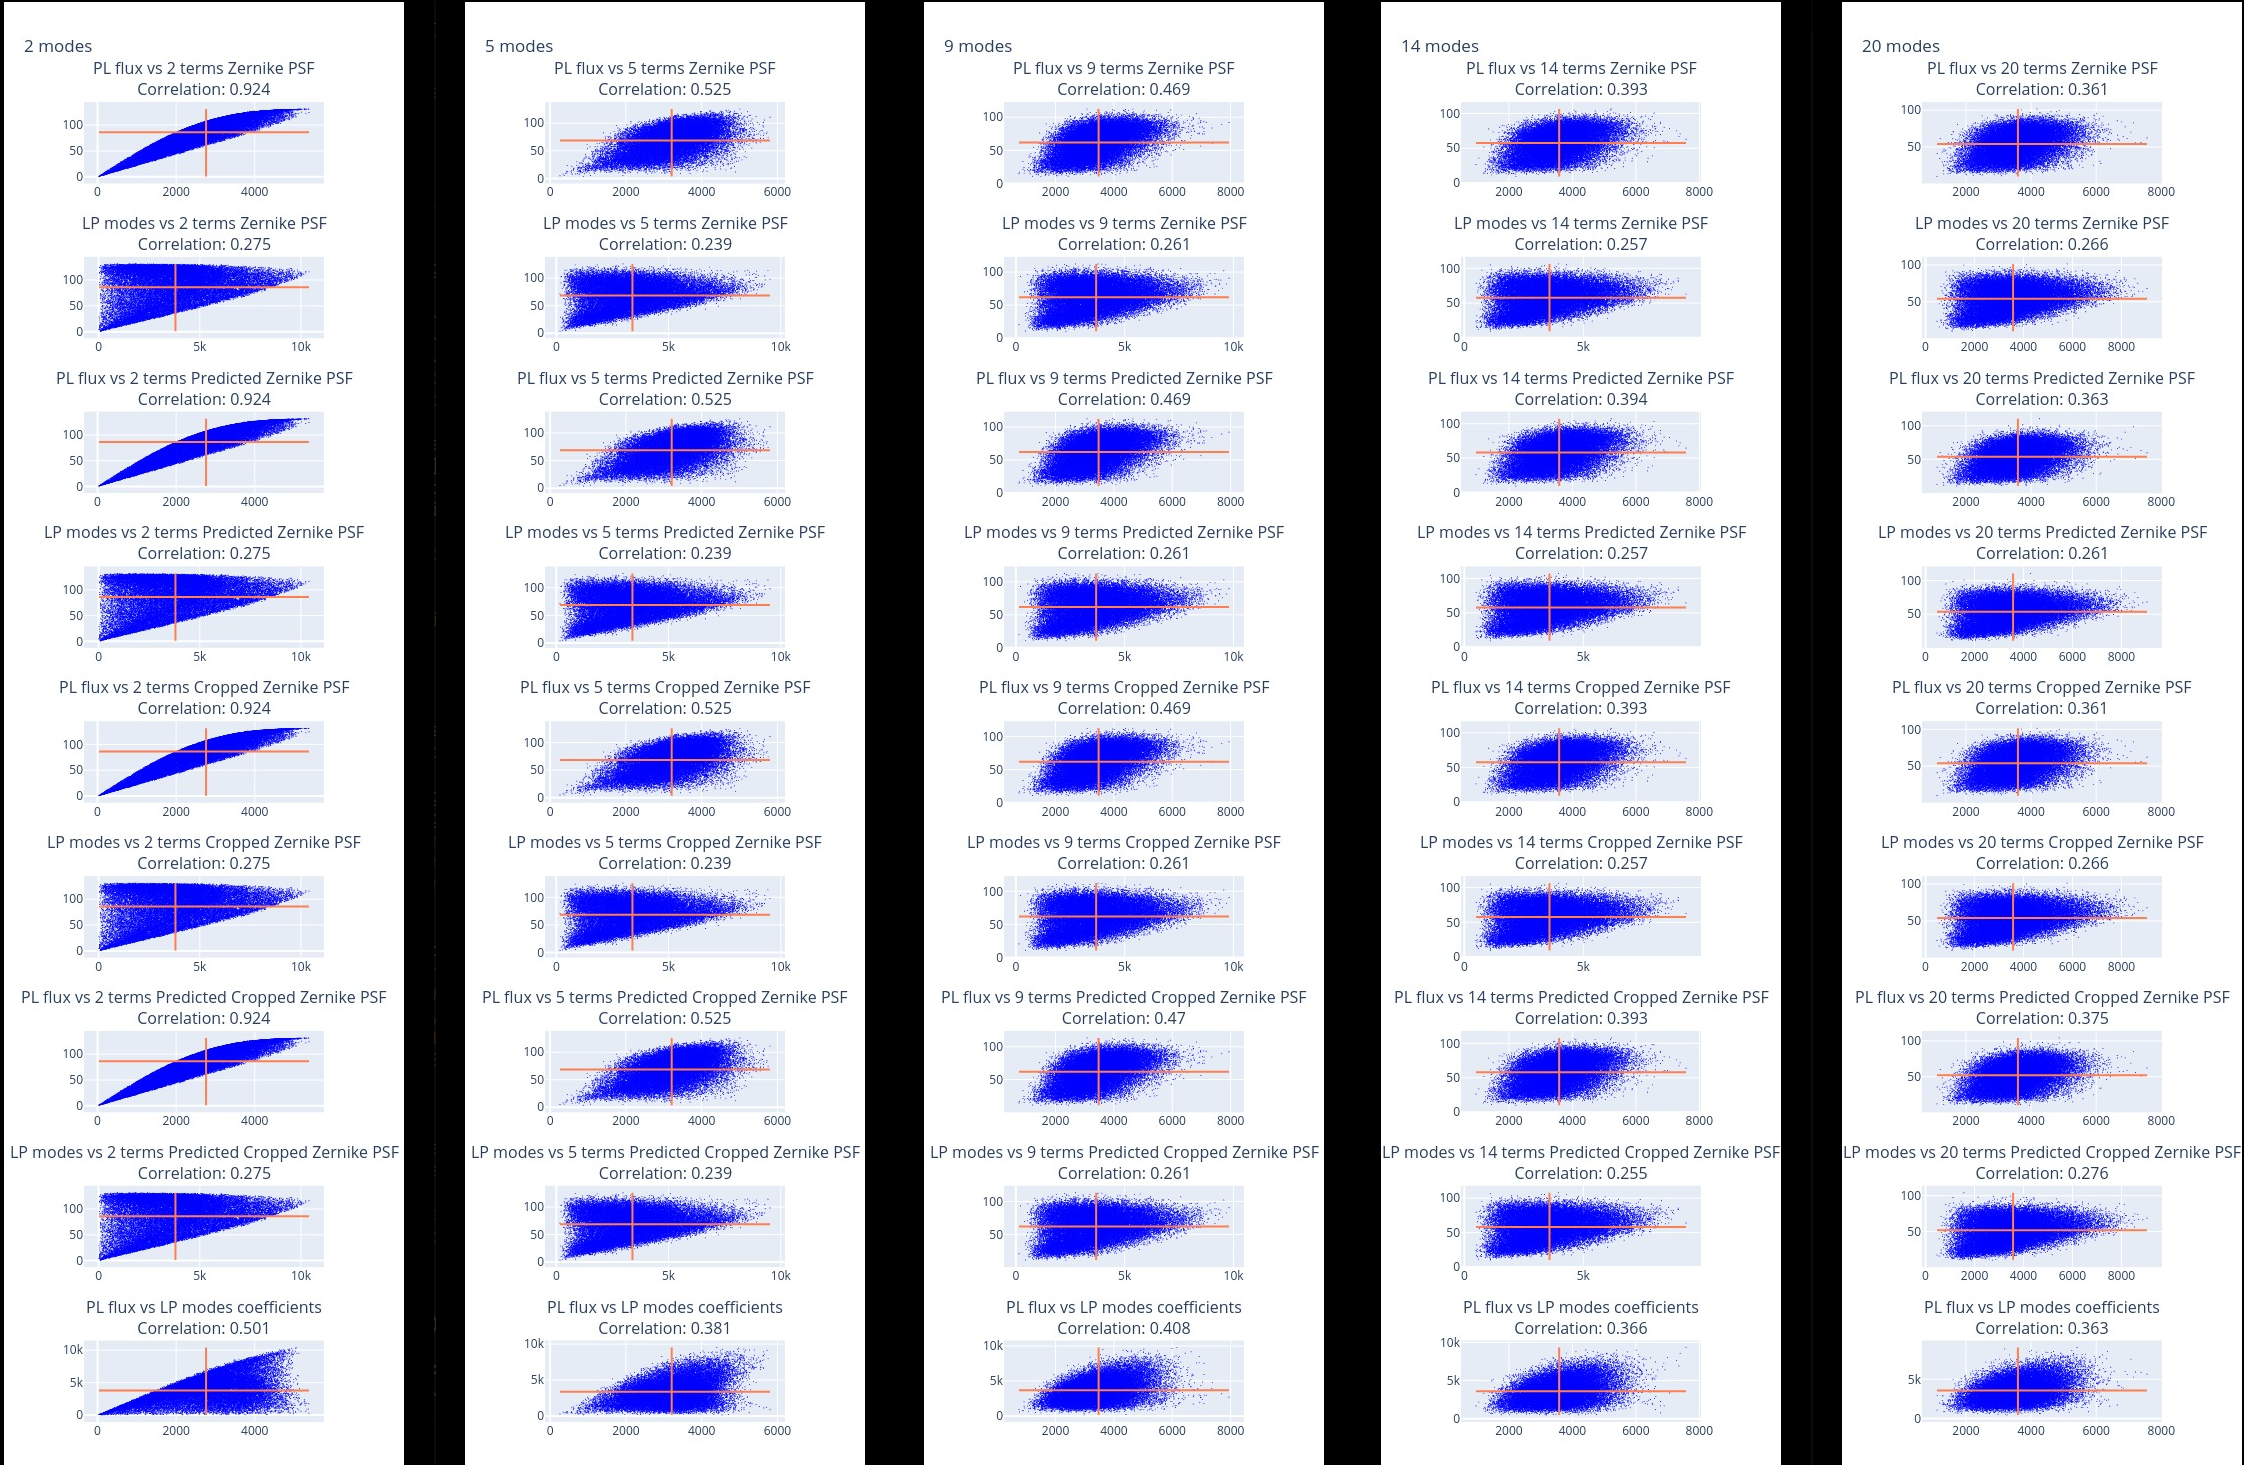
\includegraphics[scale=0.22]{pid-euclideandistanceszernike.png}
			\caption{Euclidean distances relationship between the Zernike PSFs datasets}
		\end{figure*}
		
		\begin{figure*}[ht!]
			\centering
			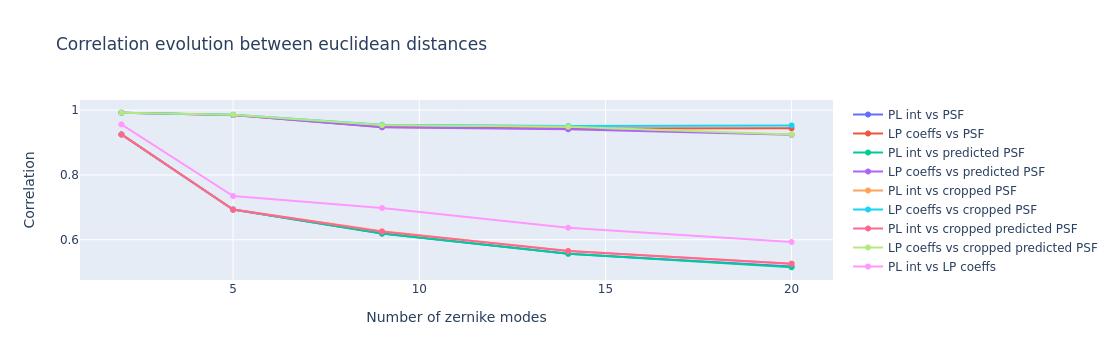
\includegraphics[width=\textwidth]{pid-euclideandistancesevolucionzernikedatasets.png}
			\caption{MSE evolution over the Zernike PSFs datasets}
		\end{figure*}
		
	\subsubsection{Analysis}
		\begin{itemize}
			\item The correlations between PSF distances and PL flux distances decay as the number of modes increases while the correlation between PSF distances and LP mode coefficients from the overlap integral are constant.
			\item The predicted psfs from the train datasets create a similar cloud of points to the original psfs which indicates that the models are capturing the information of the PL.
			\item The model trained for the dataset of 2 zernike terms PSF is the one that has the most overfit as the table shows (False, False, None indicate that no dropout, no batch normalization and no regularizer has been used), the validation mse just flatlines over the training.
			
			\item For 5 terms PSFs on the overfitting is reduced significantly although it increases with the number of zernike terms used. When using 20 terms the validation mse flatlines again.
			
			\item PL intensities vs PSF datasets evolution is practically the same for original, predicted, cropped and cropped predicted datasets. This indicates that the models are capturing accurately the relationship existing between the original PSF datasets and PL intensities datasets.
			
			\item LP coeffs vs PSF datasets evolution is practically the same for original, predicted, cropped and cropped predicted datasets.
		\end{itemize}
    
    
     
		\FloatBarrier